% !TEX root = thesis.tex

\section{Results}\label{sec:results}
\subsection{Participants}
From the 38 individuals that participated in this experiment 16 were excluded from data analysis altogether.
8 participants were excluded because their driving behavior was not indicative of an actual attempt to perform the task.
8 additional participants were excluded due to an error in the experiment, leading to the trials being too short.
This altered the task considerably and therefore we cannot compare the behavior of these participants to others.
Thus, task error was determined for 22 participants (see \citealp{DeMooij2021}). 

For eye-tracking analysis specifically, 6 more participants were excluded as their eye-tracking data were incomplete. 
This leaves us with 16 participants for eye-tracking analysis.
Finally, for the analysis of lane deviation (see \citealp{Kelapanda2021}) 15 participants were excluded because of missing data, leaving 7 participants for analysis.

\subsection{Driving behavior}
Figures~\ref{fig:errors} (from \citealp{DeMooij2021}) and~\ref{fig:lane-deviation} (from \citealp{Kelapanda2021}) show behavioral results.

\begin{figure}
  \centering
  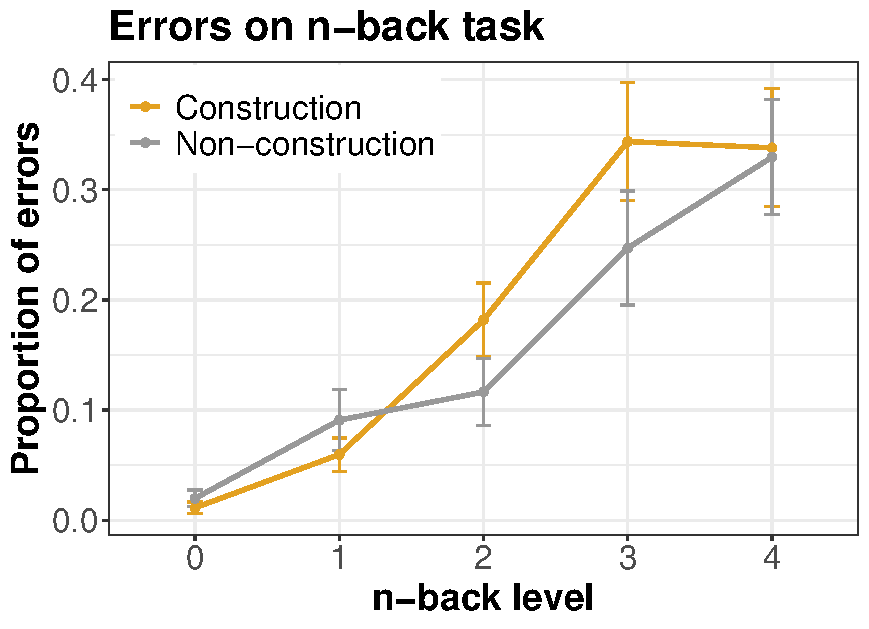
\includegraphics[width=7.5cm]{images/error_rates.pdf}
  \caption{Errors on the \textit{n}-back task (\textit{n}\ =\ 22); bars represent standard error.}
  \label{fig:errors}
\end{figure}

\begin{figure}
  \centering
  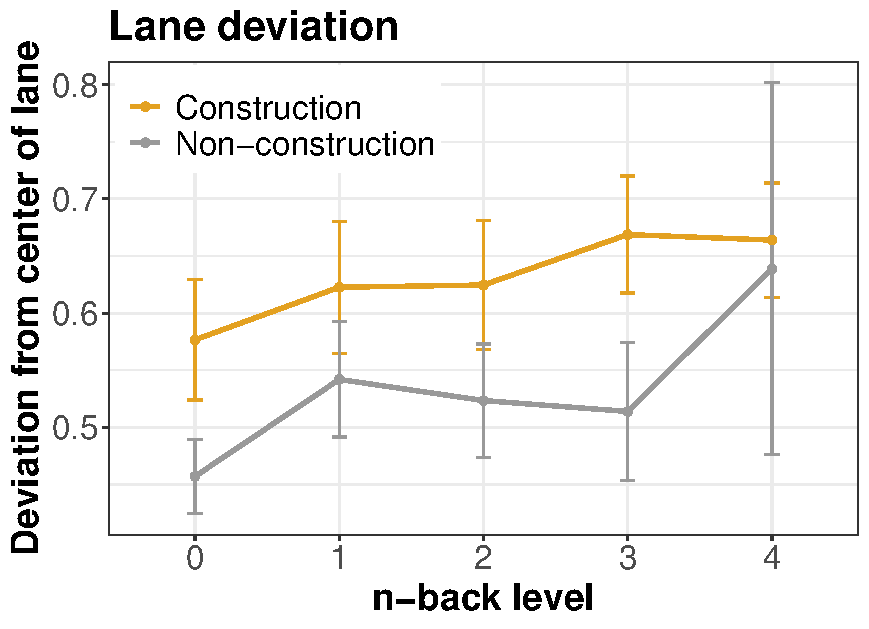
\includegraphics[width=7.5cm]{images/lane_deviation.pdf}
  \caption{Lane deviation (\textit{n}\ =\ 22); bars represent standard error.}
  \label{fig:lane-deviation}
\end{figure}

\begin{figure}
  \centering
  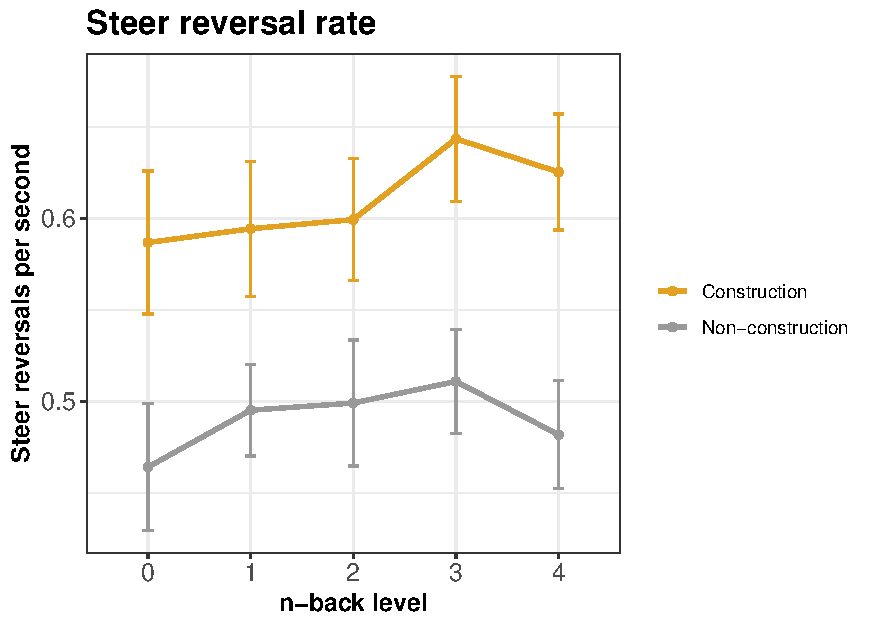
\includegraphics[width=7.5cm]{images/steer_reversal.pdf}
  \caption{Steer reversal (\textit{n}\ =\ 7); bars represent standard error.}
  \label{fig:steer-reversal}
\end{figure}

\subsection{Pupil size}
Figure~\ref{fig:ps-speed-sign} shows how the pupil size of participants changed within a trial.
There is a visible distinction between change in pupil size for low \nback levels (\(n = 0,1,2\)) and high \nback levels (\(n = 3,4\)):
whereas high \nback levels show a peak in pupil size, low \nback levels show a decline from the start of the task.
This difference, which can be characterized as an interaction between \nback level and speed sign number on pupil size, is significant according to an ANOVA with repeated measures [\(F(4,2536)=7.42,\ p < .001\)].

\begin{figure}
  \centering
  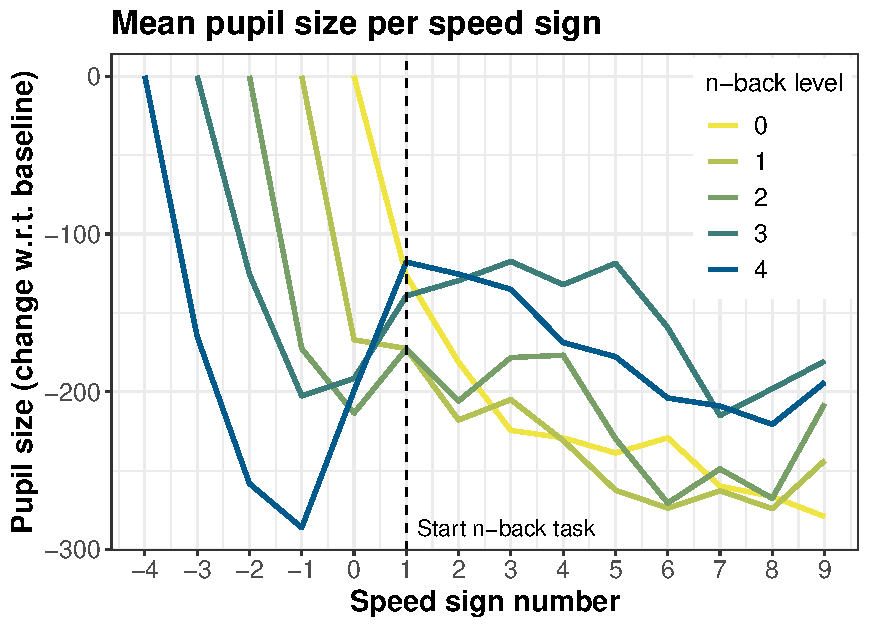
\includegraphics[width=7.5cm]{images/speed_sign_nback.pdf}
  \caption{Mean pupil size over the period between the appearance of two speed signs (\textit{n}\ =\ 25).
  The dashed vertical line indicates the moment that participants need to start regulating their speed according to the speed signs.}
  \label{fig:ps-speed-sign}
\end{figure}

Figure~\ref{fig:mean-ps} shows the mean pupil size over an entire trial. 
It suggests that there is no effect of \nback level on pupil size within the non-construction trials.
For the construction trials there seems to be an increase of pupil size by \nback level more so than for non-construction trials.
However, this suggested interaction between \nback level and construction on pupil size is not significant [\(F(4,216)=1.50,\ p=.20\)].
Disregarding the difference between construction and non-construction we do find a marginally significant effect of \nback level on pupil size [\(F(4,221)=2.39,\ p=.052\)].

\begin{figure}
  \centering
  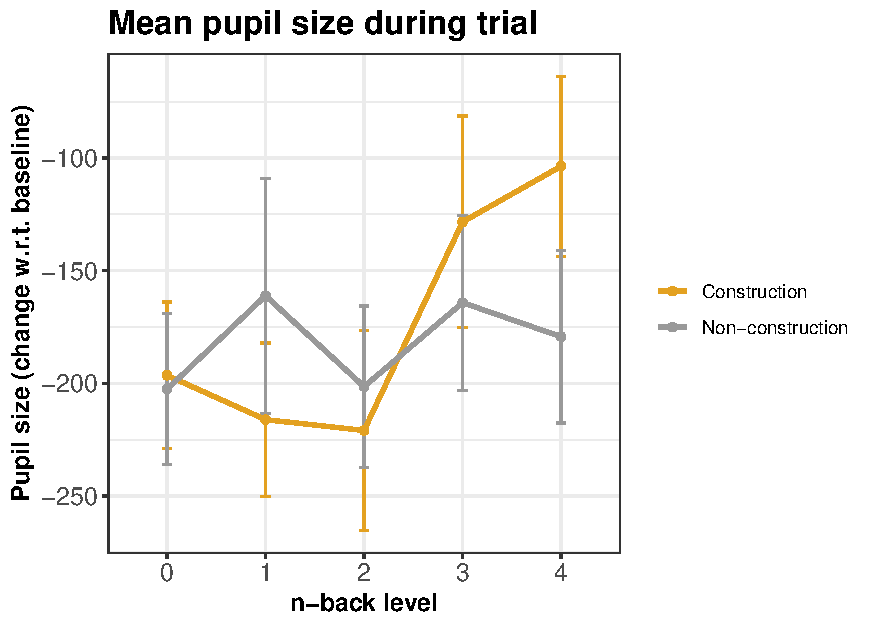
\includegraphics[width=7.5cm]{images/pupil_size_interaction.pdf}
  \caption{Mean pupil size during trial (\textit{n}\ =\ 16); bars represent standard error.}
  \label{fig:mean-ps}
\end{figure}

\subsection{Fixations on speedometer}
Figure~\ref{fig:fix-speedometer} shows the number of fixations on the speedometer as a percentage of the total number of fixations for a trial.
Like this figure suggests, there is a significant negative correlation between \nback level and fixations on the speedometer [\(F(4,221)=84.72,\ p<.001\)] 
and no effect of construction an interaction between \nback and construction. 

\begin{figure}
  \centering
  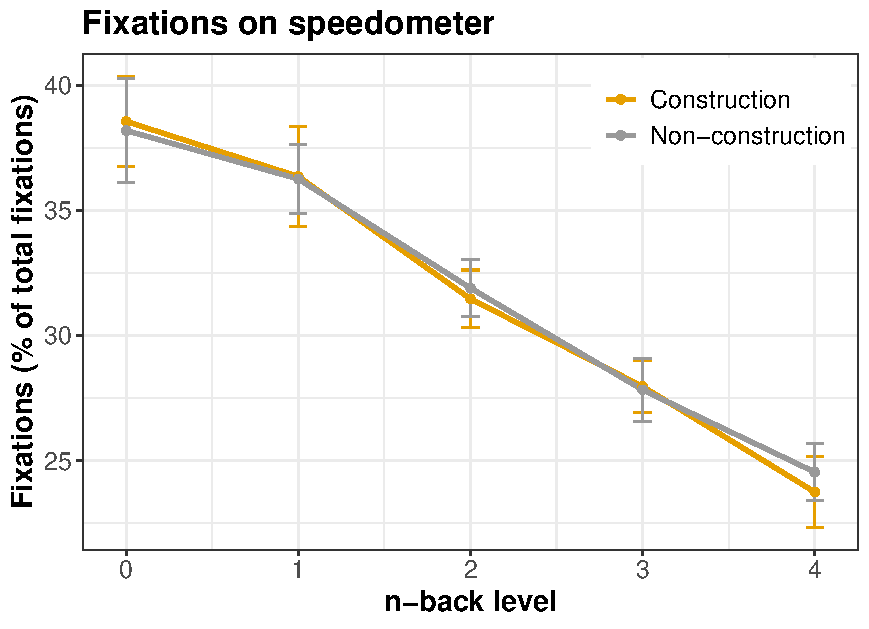
\includegraphics[width=7.5cm]{images/speedometer_interaction.pdf}
  \caption{Number of fixations on the speedometer as a percentage of the total number of fixations for that trial (\textit{n}\ =\ 16); bars represent standard error.}
  \label{fig:fix-speedometer}
\end{figure}